% !TEX TS-program = XeLaTeX
% use the following command:
% all document files must be coded in UTF-8
\documentclass[portuguese]{textolivre}
% build HTML with: make4ht -e build.lua -c textolivre.cfg -x -u article "fn-in,svg,pic-align"


\usepackage{float}
\usepackage{amsmath}
\usepackage{esvect}
\usepackage{verbatim}
\usepackage{url}
\usepackage{algorithm,algorithmic}
\usepackage{enumitem}
\usepackage{booktabs}
\usepackage{booktabs,tabularx}
\usepackage{subcaption}
\usepackage{graphicx}
\usepackage{caption}

\journalname{Texto Livre}
\thevolume{16}
%\thenumber{1} % old template
\theyear{2023}
\receiveddate{\DTMdisplaydate{2022}{10}{3}{-1}} % YYYY MM DD
\accepteddate{\DTMdisplaydate{2022}{12}{21}{-1}}
\publisheddate{\DTMdisplaydate{2023}{1}{19}{-1}}
\corrauthor{Frederico Araújo Durão}
\articledoi{10.1590/1983-3652.2023.41397}
%\articleid{NNNN} % if the article ID is not the last 5 numbers of its DOI, provide it using \articleid{} commmand 
% list of available sesscions in the journal: articles, dossier, reports, essays, reviews, interviews, editorial
\articlesessionname{articles}
\runningauthor{Santos e Durão} 
%\editorname{Leonardo Araújo} % old template
\sectioneditorname{Daniervelin Pereira}
\layouteditorname{Leonado Araújo}



\title{Um sistema de recomendação de rotas turísticas baseado em filtragem colaborativa}
\othertitle{A tourist route recommender system based on collaborative filtering}
% if there is a third language title, add here:
%\othertitle{Artikelvorlage zur Einreichung beim Texto Livre Journal}


\author[1]{Suzanne Loures Santos \orcid{0000-0003-3251-4850}\thanks{Email: \href{mailto:suzanne.loures@ufba.br}{suzanne.loures@ufba.br}}}
\author[1]{Frederico Araújo Durão\orcid{0000-0002-7766-6666}\thanks{Email: \href{mailto:fdurao@ufba.br}{fdurao@ufba.br}}}
\affil[1]{Universidade Federal da Bahia, Instituto de Computação, Salvador, BA, Brasil.}

\addbibresource{article.bib}
% use biber instead of bibtex
% $ biber article

% used to create dummy text for the template file
\definecolor{dark-gray}{gray}{0.35} % color used to display dummy texts
\usepackage{lipsum}
\SetLipsumParListSurrounders{\colorlet{oldcolor}{.}\color{dark-gray}}{\color{oldcolor}}

% used here only to provide the XeLaTeX and BibTeX logos
\usepackage{hologo}

% if you use multirows in a table, include the multirow package
\usepackage{multirow}

% provides sidewaysfigure environment
\usepackage{rotating}

% CUSTOM EPIGRAPH - BEGIN 
%%% https://tex.stackexchange.com/questions/193178/specific-epigraph-style
\usepackage{epigraph}
\renewcommand\textflush{flushright}
\makeatletter
\newlength\epitextskip
\pretocmd{\@epitext}{\em}{}{}
\apptocmd{\@epitext}{\em}{}{}
\patchcmd{\epigraph}{\@epitext{#1}\\}{\@epitext{#1}\\[\epitextskip]}{}{}
\makeatother
\setlength\epigraphrule{0pt}
\setlength\epitextskip{0.5ex}
\setlength\epigraphwidth{.7\textwidth}
% CUSTOM EPIGRAPH - END

\begin{document}
\maketitle

\begin{polyabstract}
\begin{abstract}
Planejar uma viagem, seja como turista ou a trabalho, pode não ser uma tarefa simples. Comprar passagens, encontrar acomodações disponíveis, selecionar lugares para conhecer, todo esse processo pode ser muito exaustivo considerando a quantidade de plataformas \textit{online} que oferecem serviços no âmbito turístico e a sobrecarga de informações em buscadores na Web. Sistemas de Recomendação entram nesse contexto, para filtrar as informações e sugerir dados relevantes para o usuário. Este artigo propõe um sistema de recomendação de rotas turísticas, que visa auxiliar um viajante a encontrar pontos turísticos relevantes de acordo com suas preferências e interesses.

\keywords{Sistema de recomendação \sep Pontos de interesse \sep Turismo \sep Rotas}
\end{abstract}

\begin{english}
\begin{abstract}
Planning a trip, whether as a tourist or work, may not be a simple task. Buying tickets, finding accommodations available, and selecting places to visit, this whole process can be very exhausting considering the number of online platforms that offer services in the tourist scope and also the overload of information in web search engines. Recommender Systems enter this context to filter information and suggest relevant data for the user. This article proposes a tourist route recommendation system that aims to help travelers find relevant tourist spots according to their preferences and interests.

\keywords{Recommender system \sep Point of interest \sep Tourism \sep Route}
\end{abstract}
\end{english}
% if there is another abstract, insert it here using the same scheme
\end{polyabstract}

\section{Introdução}\label{sec-intro}
De acordo com uma pesquisa realizada por \textit{We Are Social} e \textit{Hootsuite} em 2021 \cite{hootsuite2021digital}, 4,66 bilhões de pessoas em todo o mundo usam a Internet. Deste total, 4,2 bilhões usam mídias sociais, e esse número cresceu 490 milhões nos últimos 12 meses. O número de usuários de mídia social é equivalente a mais de 53\% da população mundial. O tempo médio gasto é de quase 7 horas por dia usando a Internet em todos os dispositivos, o que equivale a mais de 48 horas por semana \textit{online} \cite{WeAreSocial}.

A quantidade de pessoas \textit{online} e a rapidez com que são disseminadas as informações na Internet gerou um excesso de dados disponíveis na Web. Devido a essa sobrecarga de informação, surgiu a necessidade de filtrar informações irrelevantes apresentadas para o usuário. Uma das possibilidades de sobrecarga de informação nas mídias sociais ocorre quando um usuário, em um dado momento, acessa uma página inicial sobre rotas turísticas e depara-se com anúncios de bens de consumo de alto custo que não se relacionam com seu perfil. Outro exemplo são plataformas de \textit{stream} de música que possuem grande quantidade de músicas sem recomendações personalizadas ao usuário, o que dificulta o encontro de \textit{playlists} de sua preferência. Cenário comum igualmente ocorre quando há buscas em que os resultados ficam fora do contexto, o que torna a busca imprecisa, como é o caso de um usuário que busca por 'bateria" em um \textit{e-commerce} no qual está acostumado a comprar pilhas e obtém como retorno de baterias de instrumentos musicais ou baterias de automóveis.

Sistemas de Recomendação aparecem como uma solução para exercer a tarefa de entregar ao usuário informação de acordo com suas preferências realizando uma filtragem de informações que auxiliam a encontrar o que é relevante em um grande espaço de informações complexos \cite{DiNoia2015}.

A Filtragem Colaborativa é uma técnica de recomendação que consiste em recomendar ao usuário ativo itens que usuários com gostos similares avaliaram positivamente no passado. A filtragem colaborativa é considerada a técnica em sistemas de recomendação mais popular e mais largamente implementada \cite{Ricci:2010:RSH:1941884}.

As recomendações são amplamente utilizadas por \textit{sites} e plataformas de comércio eletrônico a fim de obter um ganho significativo ao recomendar produtos e serviços direcionados ao perfil do cliente. Nesse contexto temos o \textit{e-tourism} que é definido como uma cadeia de recomendação e planejamento turístico para auxiliar os usuários na organização de uma agenda de lazer e turismo \cite{sebastia2009tourism}.

Atualmente existe uma ampla variedade de sites e plataformas que auxiliam os viajantes a realizar o ciclo essencial que compõe uma viagem. Como exemplos pode-se citar: \textit{Airbnb}, \textit{TripAdvisor}, \textit{Expedia}, \textit{Skyscanner} e outros. Esses \textit{sites} auxiliam os turistas a conhecer pontos turísticos importantes, porém nem sempre as pessoas viajam a turismo, podendo ser a trabalho ou visita a familiares. Com uma agenda corrida, não conseguem desfrutar do que a cidade tem para oferecer. Para esses perfis, este trabalho propõe uma solução de recomendação de rotas baseada na preferência de usuário por pontos turísticos, inclusive para residentes locais. 

Considere uma pessoa visitando pela primeira vez uma determinada cidade, e que esta deseje conhecer os principais pontos turísticos. Considere também que do aeroporto até o seu hotel, localizado no centro, são aproximadamente 30 minutos com três opções de rotas: uma que passa por um mirante e um conjunto de bares, uma segunda opção com um museu e uma praça, e uma terceira via com praias. A melhor rota a ser seguida seria aquela que prioriza seus interesses. Um dos problemas nesse contexto é a falta de conhecimento das preferências do turista. Alguns podem preferir monumentos outros preferem região de praia, ou seja, a relevância dos pontos sugeridos deve ser de acordo com o perfil do visitante. 

A fim de sanar o problema descrito acima, este trabalho propõe o desenvolvimento de um sistema de recomendação de rotas turísticas que auxilie a locomoção e maximização da exploração geográfica local para o turista. Com o sistema proposto, será possível sugerir a visitação de pontos turísticos de acordo com o perfil do usuário. Para isso será necessário: mapear todas as rotas possíveis entre o ponto de partida e o destino; identificar pontos turísticos ao redor das rotas disponíveis; recomendar a melhor rota de acordo com as avaliações de outros usuários com perfil similar.

Este artigo é organizado da seguinte forma: a \Cref{sec_2} apresenta o referencial teórico da área de Sistemas de Recomendação, a \Cref{sec_3} apresenta conceitos fundamentais de \textit{E-Tourism}, a \Cref{sec_4} discute os trabalhos relacionados, a \Cref{sec_5} apresenta a proposta em detalhes, a \Cref{sec_6} apresenta a avaliação experimental e a \Cref{sec_7} conclui o trabalho.

\section{Sistemas de recomendação}\label{sec_2}

Sistemas de Recomendação são ferramentas e técnicas de \textit{software} que fornecem sugestões de itens que são mais prováveis de interesse para um usuário específico \cite{ricci2015recommender}. Para \textcite{lu2012recommender}, o objetivo de um sistema de recomendação é fornecer listas de objetos ``recomendados” personalizados para seus usuários. Para este fim, avaliações podem ser preditas ou, alternativamente, notas podem ser atribuídas a objetos ainda desconhecidos para um determinado usuário.

Sistemas de Recomendação são largamente utilizados no comércio eletrônico, entretenimento, consumo de conteúdo, indústria de serviço, entre outros. Esses podem ser encontrados em muitas aplicações atuais que entregam uma enorme coleção de itens recomendados ao usuário final, utilizando uma combinação de abordagens baseada em conteúdo, filtragem colaborativa e em conhecimento \cite{Ricci:2010:RSH:1941884}.
Para que seja possível prever se um item possui relevância para determinado usuário, o sistema deve ser capaz de prever ou comparar a significância dos itens para poder sugeri-lo. Existem várias técnicas propostas como base para um sistema de recomendação. A diferença é conduzida por suas fontes de dados, de onde vêm os dados necessários para gerar as recomendações. Em alguns sistemas, esses dados podem ser a preferência de outros usuários \cite{Burke2007}, em outros são as descrições do que compõem o item. A seguir serão detalhadas essas duas técnicas.


\subsection{Recomendação baseada em conteúdo}
Abordagens baseadas em conteúdo precisam do conhecimento das características dos itens para gerar recomendações \cite{bozo2016metadata}. Sistemas de Recomendação baseados em conteúdo recomendam itens similares àqueles que um usuário preferiu no passado, ao passo que sistemas que implementaram a técnica de recomendação colaborativa identificam usuários que possuem preferências similares a outros e sugerem itens que eles têm preferido \cite{Lops2011}.

A utilização de recomendação baseada em conteúdo tem foco na análise de um conjunto de descrições dos itens previamente classificados pelo usuário \textit{u}, para assim construir um perfil ou modelo de interesses do usuário baseado nas características dos itens classificados \cite{Mladenic:1999}. O modelo é uma representação estruturada das preferências do usuário adaptado para encontrar e recomendar novos itens que possam ser de seu interesse. O processo de recomendação consiste em comparar os atributos do modelo do usuário com os atributos de um item. O resultado é um julgamento de relevância que representa os níveis de interesse do usuário naquele item. Se um modelo reflete com precisão as preferências do usuários, apresentará grande vantagem \cite{Lops2011}. 

\subsection{Recomendação baseada em filtragem colaborativa}
Na filtragem colaborativa, o sistema recomenda ao usuário ativo itens pelos quais usuários com perfis similares se interessaram no passado. A semelhança de gostos de dois usuários é calculada baseada na similaridade do histórico de classificações dos usuários \cite{Ricci:2010:RSH:1941884}. Por exemplo, na \Cref{fig-img-001}, há um perfil de usuário principal e outros usuários considerados similares. O sistema de recomendação irá listar os itens mais relevantes para o usuário principal com base nas avaliações dos demais usuários. 

\begin{figure}[htbp]
\centering
\begin{minipage}{.8\textwidth}
 \includegraphics[width=\textwidth]{imagens/fig-001.jpg}
 \caption{Representação do funcionamento utilizando filtragem colaborativa.}
 \label{fig-img-001}
 \source{Autoria própria.}
\end{minipage}
\end{figure}


A ideia central é que a nota de um usuário \textit{u} para um novo item \textit{i} é mais provável de ser parecida com a de outro usuário \textit{v}, se \textit{u} e \textit{v} classificaram outros itens de maneira equivalente. De modo similar, é provável que \textit{u} classifique dois itens \textit{i} e \textit{j} de forma semelhante, se outros usuários têm feito classificações similares para esses dois itens \cite{Ricci:2010:RSH:1941884}. Em \textcite{Burke2002,Burke2007}, tem-se que os métodos de filtragem colaborativa podem ser divididos nas duas classes gerais baseados em \textit{vizinhança} e \textit{modelo}. 

\subsubsection{Baseado em memória ou vizinhança}
Na filtragem colaborativa baseada em vizinhança, as classificações usuário-item armazenadas no sistema são utilizadas diretamente para predizer classificações para novos itens. Isto pode ser feito de duas maneiras conhecidas como recomendação \textit{user-based} ou \textit{item-based} \cite{Ricci:2010:RSH:1941884}. De acordo com \textcite{cazella2010ciencia} a técnica de filtragem colaborativa baseada em vizinhança segue basicamente três passos:

\begin{enumerate}
	\item Calcular o peso de cada usuário em relação à similaridade ao usuário alvo (métrica de similaridade); 
	\item Selecionar um subconjunto de usuários com maiores similaridades (vizinhos) para considerar na predição; 
	\item Normalizar as avaliações e computar as predições ponderando as avaliações dos vizinhos com seus pesos.
\end{enumerate}

No primeiro passo, a definição da similaridade pode ser realizada através da aplicação de diversos coeficientes de similaridade como Cosseno, Pearson, entre outros \cite{cazella2010ciencia}. Várias abordagens têm sido usadas para calcular a similaridade entre usuários. Na maioria a similaridade é baseada nas avaliações de itens que ambos os usuários fizeram anteriormente. As duas abordagens mais populares são \textit{correlação} e \textit{baseado em cosseno} \cite{adomavicius2005}. Para análise de correlação, há o coeficiente de Pearson apresentado na \Cref{eq-pearson}.


\begin{equation}
\label{eq-pearson}
\textit{p} =\frac{\sum_{i=1}^{N} (x_i - \overline{x})(y_i - \overline{y})}{\sqrt{\sum_{i=1}^{N} (x_i - \overline{x})^2}.{\sqrt{\sum_{i=1}^{N} (x_i - \overline{x})^2}}}
\end{equation}

Na abordagem baseada em cosseno, os dois usuários x e y são tratados como dois vetores no espaço \textit{m}-dimensional, onde \(m = | S_{xy} |\). Então, a semelhança entre dois vetores pode ser medida calculando o cosseno do ângulo entre eles.

%\begin{equation}
%\label{CosenoEquacao}
%sim(x, y) = \cos(\vv{x} ,\vv{y} )= \frac{\vv{x} . \vv{y}}{||\vv{y}||_2 . %||\vv{y}||_2} =\frac{\sum_{s \in S_{xy}}^{r_{x,s} r_{y,s}}}{\sqrt{\sum_{s %\in S_{xy}}^{r^2_{x,s}}} {\sqrt{\sum_{s \in S_{xy}}^{r^2_{y,s}} }}}
%\end{equation}

%Onde \(\vv{x}\) . \(\vv{y}\) denota o produto escalar entre os vetores %\(\vv{x}\) e \(\vv{y}\). Ainda outra abordagem para medir a semelhança entre %usuários usa a medida de diferença quadrática média \cite{adomavicius2005}. %Com isso vemos que sistemas de recomendação utilizam diversos cálculos de %similaridades para gerar estimativas de classificação mais eficientes e %precisas.


\subsubsection{Baseado em modelo}\label{sec:based_model}
Em contraste com os métodos baseados em memória, os métodos baseados em modelos usam uma coleção de classificações para aprender um modelo, que é então usado para fazer previsões de classificação \cite{adomavicius2005}. Algoritmos baseados em modelo usam o banco de dados para estimar ou aprender um modelo para previsões. Diversos algoritmos podem ser usados para obter os modelos, como clusterização, redes Bayesianas, regras de associação ou modelos de fatoração de matrizes \cite{breese2013empirical}. Em seguida será abordado com mais detalhes um modelo de fatoração de matrizes. Esta é a técnica que será utilizada no desenvolvimento do sistema de recomendação proposto. 

Decomposição de matrizes em valor singular ou \textit{singular value decomposition} (SVD) é uma das formas de fatoração de matrizes usadas em filtragem
colaborativa \cite{zhang2005using}. A essência do SVD é que as relações entre usuários e itens podem ser combinadas linearmente por alguns fatores. O SVD decompõe a matriz de classificações em duas matrizes \textit{low-rank} e seu produto é a matriz de classificação aproximada representada pela \Cref{eq-svd}.

\begin{equation}
\label{eq-svd}
 R \approx {U}^t V
\end{equation}
onde \(U \in {\mathbb{R}}^{l \times m} ( l << m)\) denota a  matriz de interesse da classe usuário,  \(U_{ik}\) é o grau de interesse que o usuário i tem na classe k, onde \(Sim(a,i)\) denota a similaridade entre o usuário \(a\) e o usuário \(i\). \(I(a)\) e \(I(i)\) representam os conjuntos de itens avaliados pelo usuário \(a\) e o usuário \(i\) respectivamente, \(\overline{r}_{a}\) e \(\overline{r}_{i}\) são a média das classificações dadas pelos usuários \(a\) e \(i\) \cite{yuan2019singular}. Na prática, sistemas de recomendação que utilizam decomposição de matrizes, geralmente seguem um padrão onde a matriz de classificações é fatorada em um produto de matrizes representando fatores latentes para os itens e os usuários.

\begin{figure}[htbp]
\centering
\begin{minipage}{.8\textwidth}
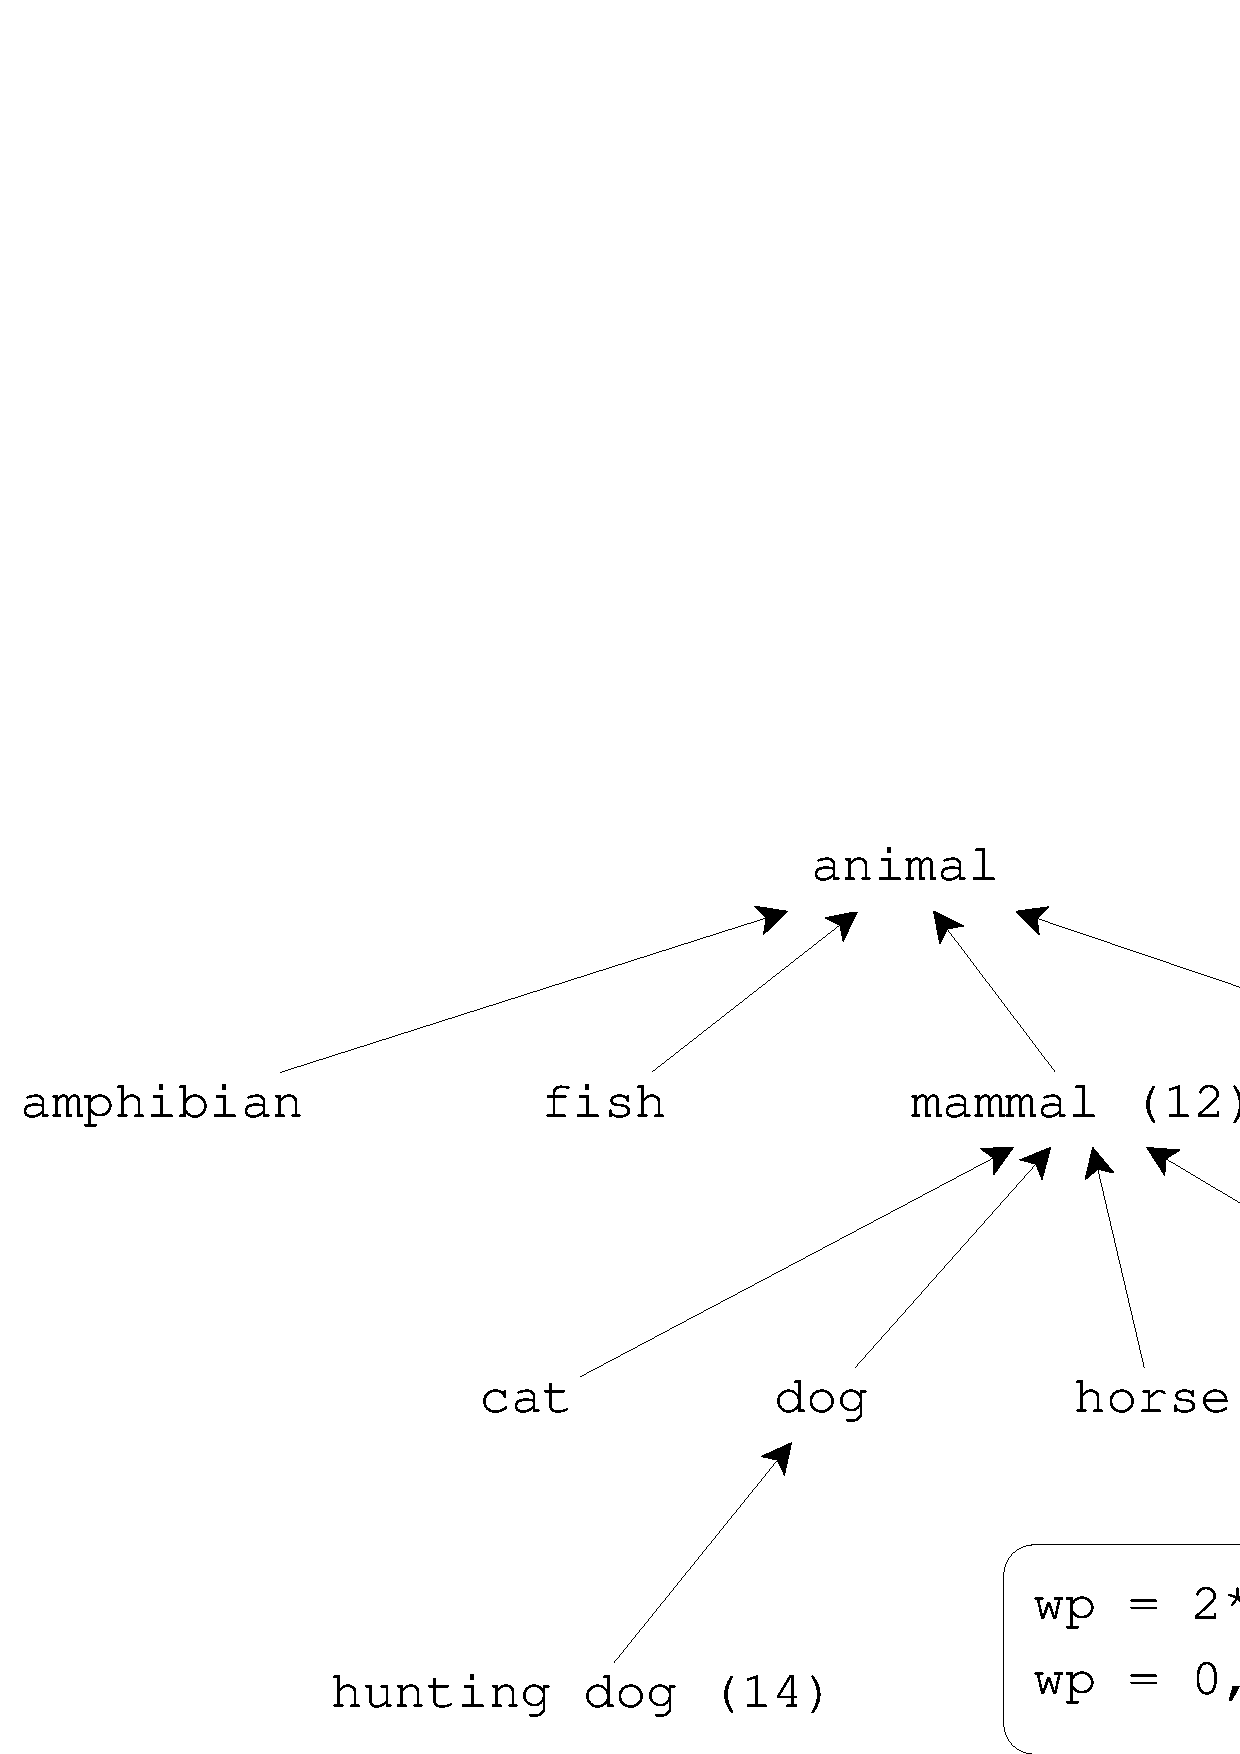
\includegraphics[width=\textwidth]{imagens/fig-002.png}
\caption{Representando classificações como um produto de matriz de fatores de item e usuário.}
 \label{fig-img-002}
\source{\cite{RecommenderSVD}}
\end{minipage}
\end{figure}

A \Cref{fig-img-002} mostra que a matriz R de classificação possui alguns espaços em branco. O algoritmo de fatoração de matrizes usa um procedimento como gradiente descendente para minimizar o erro ao prever classificações existentes usando os fatores de matriz. Podendo assim o algoritmo SVD construir uma recomendação ao “preencher as lacunas” na matriz R, prevendo as classificações que cada usuário atribuiria a cada item do conjunto de classificações \cite{RecommenderSVD}.


\section{E-Tourism}\label{sec_3}
O \textit{e-Tourism} consiste na digitalização de todos os processos e cadeias de valor da indústria do turismo, viagens e hotelaria, o que permite que as organizações maximizem sua eficiência e eficácia \cite{Moura2013}. O \textit{e-Tourism} permite que organizações gerenciem toda a operação que envolve o turismo, permitindo que dominem o \textit{e-commerce} associado ao turismo \cite{Buhalis2005}. Ele está presente em todas as camadas de planejamento e execução do processo para se realizar uma viagem, seja de cunho turístico ou a trabalho, tornando-se uma realidade de impacto no modelo tradicional do sistema turístico. Pode-se compreender o \textit{e-Tourism} como um ecossistema que está em constante mudança devido a influência de comportamento sociais e novas tecnologias. O processo de mutação é constituído por experiências do usuário e sua necessidade de partilhar informações. Para isto, são elencadas algumas etapas que compõe as três fases digitais cruciais ao realizar uma viagem \cite{Raposo2012}.

A primeira fase concentra-se em planejar a viagem e listar o que conhecer, seja um lugar ou um ponto turístico, o primeiro passo geralmente é acessar a Internet e pesquisar sobre o destino, ver as fotos dos lugares para visitar, acomodações disponíveis, comentários, vídeos, \textit{vlogs}, entres outros. Observa-se que nessa fase, o grande efeito da informação disponibilizada por outros usuários na Web que auxilia na tomada de decisão. A fase dois desse ciclo acontece durante a viagem, ela consiste em pesquisar sobre os lugares próximos a acomodação, restaurantes, rotas de passeios, \textit{shows}, eventos que estejam acontecendo durante a estadia. A fase três ocorre no período final ou retorno da viagem. Naturalmente, os usuários são levados a compartilhar, até mesmo durante a fase dois, com pessoas próximas como amigos e familiares ou seguidores em redes sociais as fotos, vídeos e opiniões sobre o lugar visitado. Essa fase tem um grande impacto social, sendo que quando compartilhamos, estamos influenciando outras pessoas.

Exemplos de sistemas comerciais de \textit{E-tourism} são: i) Airbnb\footnote{https://www.airbnb.com.br/}, site de aluguel de acomodações para curtas temporadas, muito interessante para turistas que visitam outras cidades; ii) Tripadvisor\footnote{https://www.tripadvisor.com/}, que auxilia turistas em viagens com comentários e dicas sobre pontos turísticos, restaurantes e locais para se vistiar; e o Expedia\footnote{https://www.expedia.com.br/}, que fornece opções a turistas para organizar toda a viagem, como busca de voos, aluguel de carros e hospedagem.

\subsection{Sistemas de recomendação para \textit{e-Tourism}}
Sistemas de \textit{E-Tourism} oferecem uma boa oportunidade para ajudar os visitantes, oferecendo recomendações baseadas em suas preferências e seu contexto atual \cite{BORRAS2014}. Para \textcite{loh2003tourism}, no domínio do turismo, recomendações (por humanos ou sistemas) podem indicar cidades para ir (destinos), lugares para visitar, atrações para ver, eventos, planos de viagem, roteiros, opções de hotéis, companhias aéreas etc.

Todo o ciclo que envolve a utilização de sistemas Web para auxiliar o viajante a planejar e realizar sua viagem é centralizado na busca de informações na Internet, que se torna uma tarefa complexa, pois há uma grande quantidade de dados e informações circulando a todo instante na rede. Encontrar informações pertinentes de acordo com o nosso perfil, preferências e localização no lugar visitado é um trabalho que atribuímos a plataformas que utilizem sistemas de recomendação.  

De acordo com \textcite{BORRAS2014}, a interface baseada na Web é a opção escolhida pela maioria dos sistemas, já que permite um fácil acesso de qualquer computador conectado à Web sem nenhum tipo de \textit{download}, instalação e configuração. Porém com o grande o aumento no uso de smartfones conectado à web nos últimos anos, grande parte dos recomendadores que possuem um site, também possuem aplicativos para dispositivos móveis.

A \Cref{fig:twosubs} demonstra o uso de sistemas de recomendação aplicadas no aplicativo do \textit{Google Maps}. O usuário pesquisou por "Florianópolis-Centro" e foram retornadas as coordenadas no mapa tanto quanto seções que sugerem recomendações como: melhores lugares para comer, restaurantes, bares, hotéis na região, recomendações estas que se apresentam baseadas em outros usuários ou também no perfil do usuário requisitante.  


\begin{figure}[htbp]
\begin{minipage}[t]{0.47\textwidth}
\includegraphics[width=\linewidth]{imagens/fig-003(a).png}
\subcaption{Seções de recomendações por local pesquisado.}
\end{minipage}
\hfill
\begin{minipage}[t]{0.47\textwidth}
\includegraphics[width=\linewidth]{imagens/fig-003(b).PNG}
\subcaption{Recomendação de restaurantes pela região pesquisada.}
\end{minipage}

\caption{Exemplo de recomendações pelo Google Maps.}
\label{fig:twosubs}
\source{Google Maps.}
\end{figure}


\section{Trabalhos relacionados}\label{sec_4}
Na área de Sistemas de Recomendação para o turismo encontramos diversas pesquisas e propostas que auxiliam usuários neste âmbito, com diversas técnicas de recomendação. Em \textcite{da2021sistema}, é apresentado um sistema de recomendação turístico que utiliza raciocínio baseado em casos e informações sobre geolocalização para apresentar aos usuários os pontos turísticos mais pertinentes ao seu perfil e com a localização atualizada. Esse trabalho se diferencia da nossa proposta pelo fato que usa a filtragem \textit{Knowledge Based Case}. Este método recomenda itens de acordo com os requisitos do usuário e no conhecimento de um determinado domínio para realizar recomendação enquanto a filtragem colaborativa ocorre a partir de avaliações de pontos turísticos feitas por usuários com gostos similares. Um sistema de suporte para planejamento de viagem com base em informações dinâmicas de pontos turísticos foi proposto por \textcite{hidaka2020site}. O sistema recomenda para o usuário os próximos pontos a serem visitados utilizando a seguinte metodologia: (1) Um mecanismo para adquirir informações de preferência de turistas e (2) com a localização atual um mecanismo de busca de pontos turísticos locais.

\textcite{loh2003tourism} propõem um sistema de recomendação com objetivo de ajudar os agentes de viagens a descobrir opções turísticas para os clientes, por meio de recomendações de cidades e suas atrações turísticas. Esse trabalho utiliza diversos tipos de recomendação como: \textit{Content-based, Recommendation support systems, Social data mining systems} e \textit{Collaborative filtering systems}.

No estudo realizado por \textcite{al2021hybrid} é proposta uma arquitetura e um \textit{framework} conceitual para um sistema de recomendação turístico, com base em uma abordagem de recomendação híbrida, \textit{big data} e inteligência artificial. O sistema proposto oferece outros serviços além da recomendação de uma lista de atrações adaptadas às preferências turísticas.

O sistema \textit{Multi-Agent Recommender for eTourism (MARST)} tem como objetivo recomendar serviços turísticos aos usuários, utilizando um algoritmo de filtragem colaborativa baseada em reputação (RbCF) \cite{bedi2014marst}. Assim como a proposta do nosso sistema, o MARST fornece ao usuário recomendações personalizadas e informações baseadas em localização. Entretanto, seu objetivo é recomendar serviços e não rotas turísticas e este é baseado em outra abordagem utilizando a filtragem colaborativa, com utilização de um cálculo para a reputação. O trabalho de \textcite{choudhary2019recommender} apresenta um sistema de recomendação personalizado para ajudar os usuários em destino do seu itinerário. Um modelo é projetado para sugerir os cinco melhores lugares para visita em Roma em relação à escolha feita pelo usuário. Para isso foi utilizada uma base de dados de pontos de interesse e em seguida foi coletada a preferência do usuário. Com isso foram aplicadas técnicas de mineração de dados.

Na área de recomendação de rotas turísticas, é possível encontrar algumas pesquisas recentes, como por exemplo em \textcite{10.1145/1871437.1871513} é apresentado um sistema para aplicações móveis de recomendação de rotas de viagem analisando o histórico de dados de usuários anteriores. Uma pesquisa baseada em mineração de regras de associação, que leva em consideração informações contextuais que são usadas para produzir rotas de viagem. Um outro trabalho é apresentado por \textcite{bin2019personalized}. Neste sistema de recomendação de rotas personalizadas, os pesquisadores visam inicialmente resolver os problemas de \textit{cold-start} e \textit{data sparsity} com um método para integrar dados de turismo heterogêneos coletados de sites para construir uma base de conhecimento de POI. Para isso foi utilizando um algoritmo de mineração de dados para elencar rotas candidatas de acordo com os as preferencias do turista, incluindo a duração da viagem pretendida, o tipo de acompanhante na viagem, a estação da visita e os tipos de POI preferidos. 

O trabalho de pesquisa desenvolvido por \textcite{Barbosa2022} propõe um sistema de recomendação de rotas turísticas baseado em conteúdo. Tendo como objetivo gerar recomendação de rotas de deslocamento para o usuário de acordo com o perfil em relação à semelhança descritiva entre os possíveis pontos de interesse na rota e os pontos já visitados pelo usuário. Este trabalho tem a mesma proposta do sistema apresentado nesse artigo, a diferença se encontra na abordagem de recomendação, uma vez que este trabalho relacionado utiliza uma recomendação baseada em conteúdo.  


\section{Sistema de recomendação de rotas turísticas baseado em filtragem colaborativa}\label{sec_5}

Esta seção apresenta os detalhes técnicos utilizados para o desenvolvimento deste projeto, sendo apresentada a sua arquitetura, modelo de usuário, item e recomendação.

\subsection{Arquitetura}

\begin{figure}[htbp]
\centering
\begin{minipage}{1\textwidth}
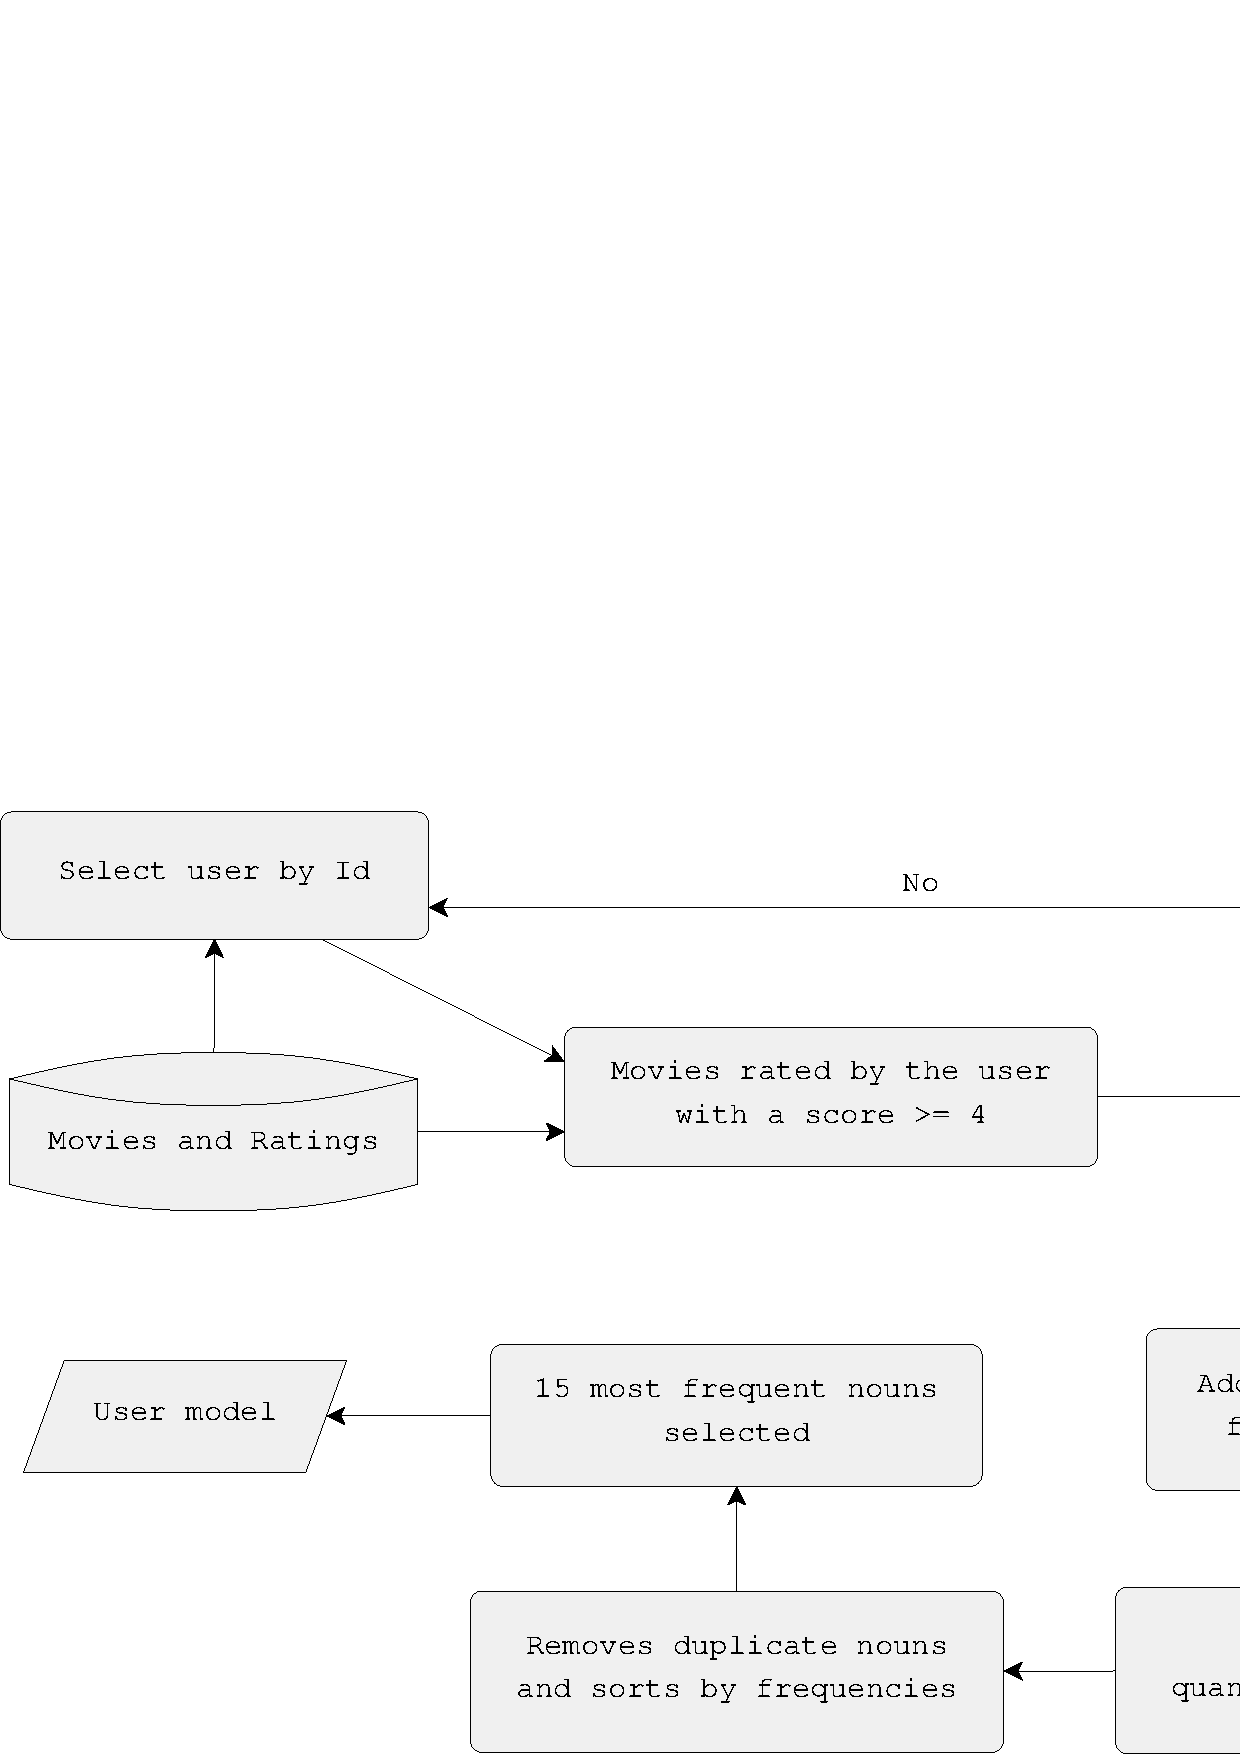
\includegraphics[width=\textwidth]{imagens/fig-004.png}
\caption{Arquitetura geral do sistema de recomendação proposto.}
\label{fig-004}
\source{Autoria própria.}
\end{minipage}
\end{figure}

A \Cref{fig-004} ilustra uma arquitetura geral para a proposta do sistema de recomendação de rotas turísticas baseado em filtragem colaborativa. A arquitetura proposta está dividida em três pilares: Recursos de dados, Sistema de Recomendação e Interface. Inicialmente na interface, o usuário informa o ponto de partida e chegada, com essa informação é realizada uma requisição para a \textit{API Google Routes} onde serão retornadas as possíveis rotas entre os pontos informados. Para cada rota serão buscados os pontos de interesse (POIs) mapeados na camada de recursos de dados, que contém o banco de dados de POIs. Desse modo, com as rotas traçadas e seus respectivos POIs, passamos para a camada onde atua o sistema de recomendação. Esta por sua vez utiliza o algoritmo de predição, baseado em fatoração de matrizes para realizar a predição de preferências para o usuário sobre um POI. A partir das preferências preditas, podemos então executar um cálculo para ranquear e recomendar a melhor rota para os usuários.

\subsection{Modelo do usuário}
Formalmente, o modelo do usuário, definido como $M_u$ e apresentado em \Cref{eq:usermodel}, é formado pela tupla %\re 
que contém o comportamento do usuário para um item, constituído por uma nota $a\in A$, escala de 0 a 5, para pontos de interesse $p \in P$. Com essa representação do modelo do usuário obtemos a sua preferência a partir dos pontos que foram mais bem avaliados.

\begin{equation}
\label{eq:usermodel}
(\forall u \in U) \quad M_{u} =  {\ \langle (p1,a1),(p2,a3),...(pn,an) \rangle}
\end{equation}

O exemplo a seguir mostra que para a usuária chamada Carla, os pontos com notas maiores são para os itens \textit{Farol da Barra} e \textit{Farol de Itapuã}. Esses dois locais são pontos turísticos da cidade de Salvador, capital do estado da Bahia.

\begin{equation}
\label{eq:usermodelexample}
M_{\text{Carla}} = \text{ (Farol Barra,5),(Farol Itapuã,4),(Praia Ondina,3),(Mirante Praia ,2)} 
\end{equation}
 
O modelo de usuário será construído com base nas informações obtidas na base de dado que contém a identificação do usuário por um identificador e a sua respectiva avaliação, uma nota entre 1 e 5 para um determinado local. Os dados são um conjunto de pontos turísticos visitados pelos usuários. Assim, é possível identificar, por exemplo, quais os pontos turísticos mais e menos bem avaliados.

\subsection{Modelo do item}
Formalmente, cada item é um ponto de interesse (museu, bar, praia, parque, etc.) $p \in P$. Cada item é formado por uma quíntupla:

\begin{equation}
\label{eq:itemmodel}
(\forall p \in P) \quad M_{p} =  {\langle  \text{UID,CAT,NAME,LAT,LONG}  \rangle }
\end{equation}

onde UID é a identificação única do item, CAT é a categoria do POI, NAME é o nome em texto atribuído, LAT e LONG são as coordenadas geográficas em latitude e longitude.

\subsection{Modelo de recomendação}
\label{sec:modelo_recomendacao}
O sistema proposto recomendará uma rota principal $r\in{R}$, dentro das possíveis rotas $R$, considerando os pontos $A$ e $B$ (partida e chegada) fornecidos pelo usuário $u\in{U}$. Esta rota será composta de pontos de interesse $p\in{r}$ que estejam próximos da rota definida.

As preferências dos usuários sobre os itens constituem uma matriz, entretanto como nem todos os usuários avaliam todos os itens, realizamos a fatoração da matriz apresentada na \Cref{sec:based_model}, a fim de reduzir a dimensionalidade, e em seguida predizer a nota que cada usuário daria a cada POI. Com o valor de cada avaliação $a \in A$ predita para o POI, podemos formular a seguinte equação para gerar uma avaliação final para cada rota: 

\begin{equation}
\label{eq:recscore}
    \mbox{recScore}(r) = \frac{\sum_{i=1}^{n}a_i}{\sum_{i=1}^{n}Pr_i}
\end{equation}

onde a soma das avaliações é dividida pela soma da quantidade de pontos $P_r$ encontrados na rota. A partir do resultado da equação, é gerada a recomendação da melhor rota para o usuário final. O algoritmo proposto neste trabalho pode ser melhor entendido através de um pseudocódigo apresentado abaixo:

\begin{algorithm}[H]
 \caption{Algoritmo de recomendação de rotas a partir de pontos de interesse}
 \label{alg:obtencao_rotas}
 \begin{algorithmic}[1]
 
 \renewcommand{\algorithmicrequire}{\textbf{Entrada:}}
 \renewcommand{\algorithmicensure}{\textbf{Saída:}}
 
 \REQUIRE $a$, $b$ sendo respectivamente os pontos de partida ($a$) e chegada ($b$)
 \ENSURE Lista de rotas possíveis entre $a$ e $b$ com os pontos de interesse encontrados 
 
 \STATE rotas $\leftarrow$ rotasGoogle(a,b)
    \FOR{rota $\in$ rotas}
    \FOR{coordenada $\in$ rota}
        \item {rota.pontosDeInterese $\leftarrow$ + pontosProximos(coordenada)}
    \ENDFOR
    \ENDFOR
    
    \FOR{rota $\in$ rotas}
    \FOR{pontoDeInteresse $\in$ rota}
        \item {rota.score $\leftarrow$  pontoDeInteresse.predict(UserId, pontoDeInteresse)}
    \ENDFOR
      \item {rota.scoreRota $\leftarrow$ recScore(rota)}
    \ENDFOR
 \end{algorithmic} 
 \end{algorithm}
 
\subsection{Recomendação em ação}\label{sec:recomendation_in_action}
A fim de ilustrar o modelo proposto, considere o seguinte cenário: Eduarda reside na cidade de Campinas - SP, tem interesse por praias e gosta de monumentos. Ela precisa viajar a trabalho para Salvador - BA, com uma estadia de 3 dias. Seu hotel fica localizado no bairro da Pituba em Salvador e ela tem que ir à reunião de trabalho localizada na Barra. Como Eduarda não terá tempo para visitar os principais pontos turísticos da cidade, ela decide utilizar o sistema proposto para saber qual melhor trajeto de maneira que possa usufruir ao máximo da sua experiência em Salvador, ainda que esteja a trabalho.


% \begin{figure}[h]
% 	\centering
% 	\includegraphics[width = 1\textwidth]{images/user-case.jpeg}
% 	\caption{Fluxo do usuário interagindo com o sistema.}
% 	\label{fig:cycle}
% \end{figure}

A \Cref{fig-005} mostra Eduarda informando a localização de partida e chegada na página de busca, a partir dessa informação serão sugeridas três rotas pela \textit{API do Google Routes}. Para cada rota, nosso algoritmo de predição retornará uma possível avaliação para cada ponto turístico encontrado. Para isso, consideramos o seguinte modelo do usuário para Eduarda:

\begin{equation}
\label{eq:usermodelexample}
M_{\text{Eduarda}} =  \text{(Praia Pituba,5),(Monumento Cleriston Andrade,4)} 
\end{equation}

\begin{figure}[htbp]
\centering
\begin{minipage}{.9\textwidth}
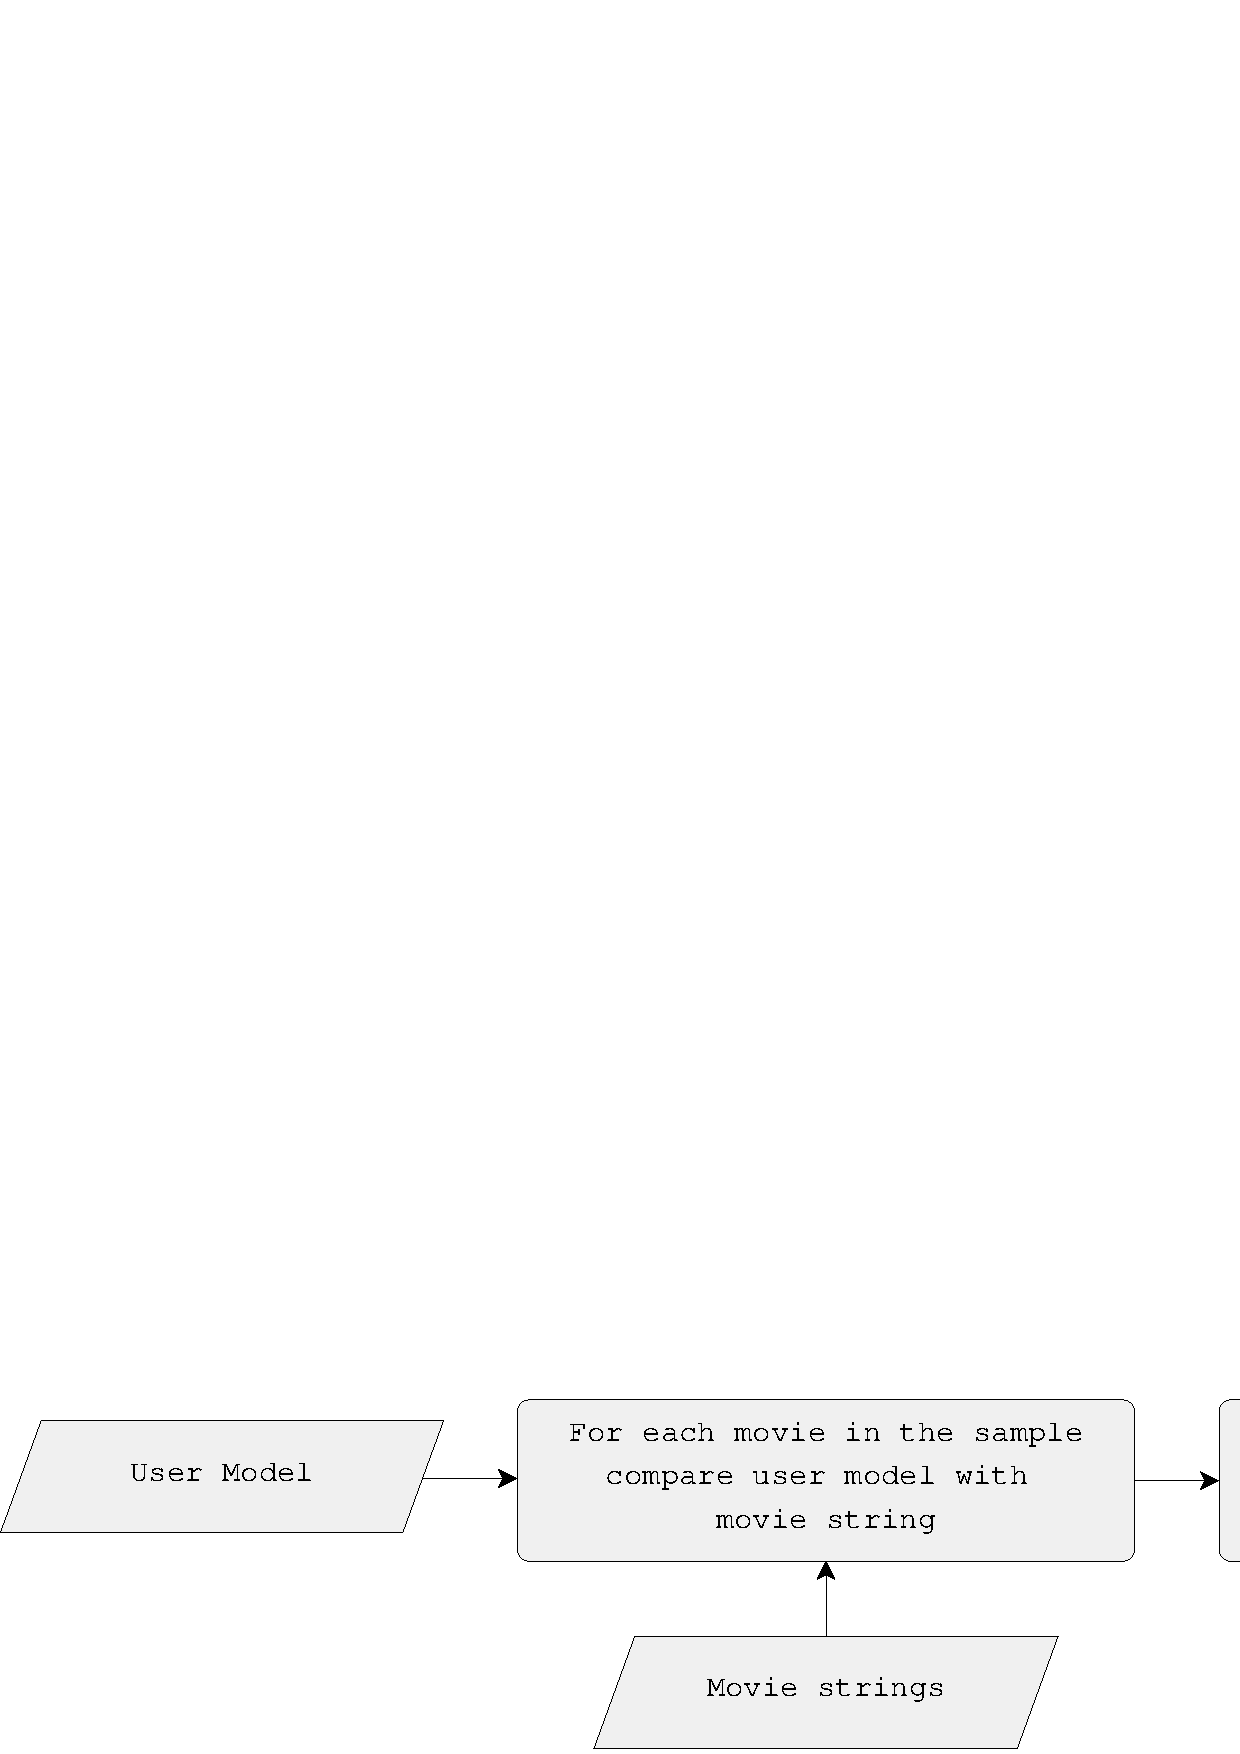
\includegraphics[width=\textwidth]{imagens/fig-005.jpeg}
\caption{Fluxo do usuário interagindo com o sistema.}
\label{fig-005}
\source{Autoria própria}
\end{minipage}
\end{figure}

Com $M_{\text{Eduarda}}$ o algoritmo SVD realizará o treinamento da base de dados de avaliações, considerando as notas anteriormente informadas por Eduarda e as avaliações dos outros usuários para pontos de interesse encontrados na rota. A partir desse treinamento, obtemos as seguintes predições apresentadas nas \Cref{tab01}, \Cref{tab02} e \Cref{tab:table3}:

%\begin{enumerate}[label=(\Alph*)]

%\item { (Praia da Pituba, 4.55), (Largo das Baianas, 4.46) (Praia de Amaralina, 4.37),(Praia do Rio Vermelho, 4.26),(Monumento As gordinhas, 4.37), (Morro do Cristo, 4.39)}
%\item { (Parque da cidade, 4.37),(Monumento Clériston Andrade, 3.36), (Monumento As gordinhas, 4.39), (Morro do Cristo, 4.39)}
%\item {(Parque da cidade, 3.37), (Morro do Cristo, 4.39) }

%\end{enumerate}

\begin{table}
\parbox[t]{.45\linewidth}{
\centering
\begin{threeparttable}
\caption{Rota A.}\label{tab01}
\begin{tabular}{ll} 
\toprule
Pontos & Avaliação \\  
\midrule   
Praia da Pituba & 4,55 \\
Largo das Baianas & 4,46 \\
Praia de Amaralina & 4,37\\
Praia do Rio Vermelho &  4,26 \\
Mon. As gordinhas & 4,37 \\
Morro do Cristo & 4.39 \\ 
\bottomrule
\end{tabular}
\end{threeparttable}
}
\hfill
\parbox[t]{.45\linewidth}{
\centering
\begin{threeparttable}
\caption{Rota B.} \label{tab02}
\begin{tabular}{ll} 
\toprule
Pontos & Avaliação \\ 
\midrule
Parque da cidade & 4,37 \\
Mon. Clériston Andrade & 3,36 \\
Mon. As gordinhas & 4,37 \\
Morro do Cristo & 4.39 \\ 
\bottomrule
\end{tabular}
\end{threeparttable}
}
\end{table}


\begin{table}[h!]
\centering
\begin{threeparttable}
\caption{Rota C.}
\label{tab:table3}
\begin{tabular}{ll} 
\toprule
Pontos & \textit{recScore} \\ 
\midrule
Parque da cidade & 4,37 \\
Morro do Cristo & 4.39 \\ 
\bottomrule
\end{tabular}
\end{threeparttable}
\end{table}

De acordo com o modelo do perfil de Eduarda, $M_{\text{Eduarda}}$, a rota recomendada será aquela que obtiver a maior avaliação a partir da \Cref{eq:recscore}. A \Cref{tab:table4} apresenta todas as avaliações finais para cada rota, após ser calculada através do \textit{recScore}.


\begin{table}[h!]
\centering
\begin{threeparttable}
\caption{Avaliações obtidas através do \textit{recScore}.}
\label{tab:table4}
\begin{tabular}{ll} 
\toprule
Nome da rota & \textit{recScore} \\ 
\midrule
Rota A & 4,40 \\
Rota B & 4,37 \\
Rota C & 4,38 \\ 
\bottomrule
\end{tabular}
\end{threeparttable}
\end{table}

É possível observar que a rota A obteve maior avaliação, sendo esta a primeira rota recomendada. A rota C por sua vez, tem apenas dois pontos turísticos que pouco exploram a cidade, porém ela é melhor avaliada do que a Rota B, que possui mais pontos de interesse do usuário como o \textit{Monumento As Gordinhas}. Portanto, nem sempre as rotas serão ranqueadas de acordo com a sua relevância para o usuário.


\section{Avaliação experimental}\label{sec_6}
Nesta seção é apresentado o processo de avaliação para validar se os objetivos iniciais previstos foram alcançados. Espera-se que, com a recomendação de rotas de pontos turísticos, o usuário possa visitar a maior quantidade de pontos de interesse dentro do seu trajeto natural, e que possua relevância de acordo com sua preferência.


\subsection{Conjunto de dados}\label{conjunto-dados}
Os experimentos foram realizados utilizando conjunto de dados \textit{Salvador Routes for Tourists}\footnote{\url{https://www.kaggle.com/datasets/ramonbrbs/salvador-routes-for-tourists}}, extraídos a partir de um estudo na área de sistemas de recomendação e obtido a partir da plataforma \textit{Kaggle}\footnote{\url{https://www.kaggle.com/datasets}}. O conjunto de avaliações contém 3240 registros de 81 usuários. O conjunto de POIs totalizam 91 pontos turísticos de Salvador-BA. A \Cref{tab:dataset} resume alguns dos campos disponíveis nas tabelas do conjunto de dados. 


\begin{table}[h!]
\caption{Resumo do conjunto de dados.}
\label{tab:dataset}
\begin{tabularx}{\linewidth}{r l X}
\toprule
Campo & Descrição\\
\midrule
UserId & Identificação única do usuário \\
PoiId & Identificação única do ponto turístico\\
Rating & Nota do usuário para o ponto turístico \\
UserScore & Ranking das preferências do usuário para uma lista de rotas recomendadas \\
RouteTitle & Ponto de partida e chegada para cada rota \\
Summary & Resumo do trajeto indicando as vias\\
\bottomrule
\end{tabularx}
\end{table}

\subsection{Metodologia}
Para coletar os dados na \Cref{conjunto-dados}, foi realizado o levantamento de informações para definir as preferências dos usuários. Membros da comunidade acadêmica do Instituto de Computação e participantes externos foram convidados para participar do experimento. O experimento foi dividido em 2 etapas: na primeira, de 29 de abril a 23 de maio de 2022, os participantes foram solicitados para avaliarem 20 pontos de interesse aleatoriamente (nota de 1 a 5). Na segunda etapa, de 30 de maio a 10 de junho de 2022, os participantes foram apresentados às rotas recomendadas entre os dois trajetos previamente traçados, e foi solicitado que ordenassem as rotas obtidas de acordo com a sua preferência pelos pontos de interesse presentes nas rotas.

Após obtenção dos dados, foi necessário o pré-processamento devido a escassez de avaliações pelos usuários. Foram removidos todos os registros cujas avaliações eram nulas para geração de um modelo ótimo de treinamento. A \Cref{tbl-tabela-6} mostra as estatísticas descritivas que incluem a tendência central, dispersão e forma da distribuição do conjunto de dados. 
\begin{table}[htpb]
\centering
\begin{threeparttable}
\caption{Estatísticas do conjunto de avaliações.}
\label{tbl-tabela-6}
\begin{tabular}{p{4cm}lll}
\toprule 
- & userId & poiId & rating \\
\midrule
count     & 510   & 510 & 510      \\
mean      & 36.184   & 3.452 & 3.390 \\
std       & 8.485 & 3.240 & 1.422     \\
min       & 19 & 3.787 & 1       \\
25\%      & 30 & 4.631 & 2         \\
50\%      & 37 & 1.818 & 4         \\
75\%      & 43 & 5.752 & 5         \\
max       & 50 & 9.655 & 5         \\
\bottomrule
\end{tabular}
\source{Autoria própria.}
\end{threeparttable}
\end{table}


%Após o tratamento de dados, foi solicitado a cada participante avaliasse rotas recomendadas para 2 trajetos, denominadas Experimento 1 e Experimento 2:
A partir do conjunto de dados de avaliações de pontos de interesse obtido na primeira etapa, a base foi submetida ao treinamento a partir do algoritmo SVD baseado em fatoração de matrizes, que extrai vetores de características latentes de usuário e item e preenche as lacunas de avaliações de usuários para itens. Assim foi possível elaborar dois experimentos utilizando o nosso resultado para ser comparado com o conjunto de avaliações de rotas obtidos na segunda etapa.


\begin{itemize}
    \item \textbf{Experimento 1} : Gerar um \textit{ranking} de recomendações de rotas a partir do trajeto: Ponto de partida: \textit{Arena Fonte Nova} e o ponto de chegada \textit{Largo de Santana (Largo da Dinha)}. 
    \item \textbf{Experimento 2} : Gerar um \textit{ranking} de recomendações de rotas para o trajeto: Ponto de partida: \textit{Farol Da Barra} e o ponto de chegada \textit{Dique do Tororó}.  
    
\end{itemize}

%\begin{figure}[htbp]
%\begin{minipage}[t]{0.47\textwidth}
%\includegraphics[width=\linewidth]{imagens/fig-006(a).png}
%\subcaption{Antes do pré-processamento.}
%\end{minipage}
%\hfill
%\begin{minipage}[t]{0.47\textwidth}
%\includegraphics[width=\linewidth]{imagens/fig-006(b).png}
%\subcaption{Após o pré-processamento.}
%\end{minipage}

%\caption{Estatísticas do conjunto de avaliações.}
%\label{fig-006}
%\source{Autoria própria.}
%\end{figure}

Para cada usuário foi aplicado o Experimento 1 e pode-se obter o \textit{recScore} para 3 rotas dentro do trajeto especificado. O \textit{ranking} foi elaborado da seguinte forma: a maior nota atribui-se ao 1º lugar, ou seja, a rota que o usuário teria como preferência, em seguida as demais em ordem decrescente 2ª e 3º lugar.
%Para cada uma das 3 rotas recomendadas foi comparado os rankings atribuídos em relação os rankings verdadeiramente avaliados.
Na \Cref{tab:table6}, podemos visualizar a lista de recomendação para o $u_{21}$, que contém a descrição da rota com as vias a serem percorridas, o \textit{recScore} e a posição na lista com \textit{Rank}.

\begin{table}[htpb]
\centering
\begin{threeparttable}
\caption{Recomendações com o Rank.}
\label{tab:table6}
\begin{tabular}{llll} 
\toprule 
UserId & Resumo  & \textit{recScore} & Rank\\
\midrule
21  & Av. Vasco da Gama e Av. Anita Garibaldi &  4,11 & 1º  \\
21 & Av. Vasco da Gama & 4,10 & 2º \\
21 & Av. Gen. Graça Lessa e Av. Vasco da Gama & 4,08 & 3º \\
\bottomrule
\end{tabular}
\source{Autoria própria.}
\end{threeparttable}
\end{table}



\subsection{Métrica de avaliação}
Existem diversas métricas que podem ser utilizadas para avaliar a assertividade de um sistema de recomendação. Para este trabalho, foi utilizado o MRR \textit{(Mean Reciprocal Rank)} a fim de responder a seguinte pergunta ``Quão longe está o item classificado em 1º lugar do item mais relevante para o usuário?". O MRR avalia a qualidade das listas de recomendação na posição top-N, medindo a distância entre o item mais relevante e o topo da lista. O MRR está definido como:
\begin{equation}
\label{eq:mrr}
\text{MRR} = {\frac{1}{|U|}\sum_{u \in U}\frac{1}{P_i}}
\end{equation}
onde $(\forall u \in U)$ a primeira ocorrência de uma recomendação relevante $p_i \in P_i$ é avaliada. No contexto desse trabalho, a fim de medir o quão distante o item recomendado está do topo da lista elaboramos a seguinte metologia para cada usuário $u_{x}$:
\begin{enumerate}

\item Procurar a rota verdadeiramente classificada como mais relevante (p@1);
\item Obter o RR ({\textit{Reciprocal Rank}})  $\frac{1}{P_i}$ ;
\item Obter o resultado com o MRR apresentado na \Cref{eq:mrr}.
\end{enumerate}

Com o intuito de ilustrar a aplicação do cálculo do MRR no contexto desse trabalho, a \Cref{tab:table7} exibe que para o usuário $u_{19}$, o item mais relevante recomendado está na p@3, sendo assim, seu RR = $\frac{1}{3}$. Para o $u_{21}$ o item mais relevante (destacado em negrito) está p@2 $\text{RR} = \frac{1}{2}$. E para o $u_{24}$ ambos itens relevantes se encontram na p@1 posição com um RR = 1. Portanto, o MRR calculado é de 0,611. No exemplo utilizado, ``Vasco", ``Graça" e ``Garibaldi" são bairros da cidade de Salvador que possuem pontos de interesse.

\begin{table}[h!]
\centering
\begin{threeparttable}

\caption{Exemplo do cálculo do MRR para 3 usuários extraídos da avaliação.}
    \label{tab:table7}
\begin{tabular}{ cccc } 
        \toprule 
            usuário & rank gerado & rank esperado & RR\\
         \midrule
         $u_{19}$  & Vasco, Graça, \textbf{Garibaldi} &  \textbf{Garibaldi}, Vasco, Graça & 1/3  \\

         $u_{21}$ & Garibaldi,\textbf{Vasco}, Graça & \textbf{Vasco}, Garibaldi, Graça & 1/2 \\
    
         $u_{24}$ & \textbf{Garibaldi}, Vasco, Graça & \textbf{Garibaldi}, Vasco, Graça & 1 \\
        \bottomrule
    \end{tabular}
\source{Autoria própria.}
\end{threeparttable}
\end{table}

\subsection{Resultados}

A métrica MRR foi utilizada para medir a assertividade do sistema, quanto à posição da rota relevante na lista recomendada em relação à lista preferencial do usuário. Os testes contam com 27 usuários e 162 avaliações. A \Cref{table-results} mostra os resultados do RR para todos os usuários para o Experimento 1 \Cref{table-results-a} %Tabela na 8a 
e Experimento 2 na \Cref{table-results-b}.% Tabela 8b.


\begin{table}[htbp]
\centering
\caption{Resultados de ambos experimentos, exibindo a possição o respectivo Reciprocal Ranking.}
\label{table-results}
\begin{minipage}[t]{0.47\textwidth}
\subcaption{Experimento 1:\\Fonte Nova -> Largo da Dinha.}
\label{table-results-a}
\centering
\begin{tabular}{ll}
\toprule
UserId  & Recp. Rank \\
\midrule
19     & 0,33    \\
21     & 0,5      \\
22    & 0,5      \\
24     & 1       \\
25    & 0,5      \\
26    & 0,5      \\
27    & 1         \\
30    & 0,33       \\
31     & 0,5       \\
32    & 1          \\
33    & 0,33       \\
34     & 0,33      \\
35     & 1         \\
36     & 0,5      \\
37     & 0,33      \\
38     & 0,33      \\
39     &  1        \\
40     &  1        \\
41     &  0,33        \\
42     &  0,33        \\
43     &  1        \\
44     &  0,33        \\
45     &  0,5        \\
46     &  0,33        \\
48     &  0,5        \\
49     &  1        \\
50     &  0,5        \\
\bottomrule
\end{tabular}
\end{minipage}
\hfill
\begin{minipage}[t]{0.47\textwidth}
\centering
\subcaption{Experimento 2:\\Farol da Barra -> Dique do Tororó.}
\label{table-results-b}
\begin{tabular}{ll}
\toprule
UserId & Recp. Rank \\
\midrule
19     & 1   \\
21     & 1      \\
22    & 0,5      \\
24     & 1       \\
25    & 0,33      \\
26    & 1       \\
27    & 0,33         \\
30    & 0,5       \\
31     & 0,33       \\
32    & 0,5          \\
33    & 1       \\
34     & 1      \\
35     & 1         \\
36     & 0,5      \\
37     & 0,33      \\
38     & 0,33      \\
39     & 0,33        \\
40     &  1        \\
41     &  1        \\
42     &  1        \\
43     &  0,5        \\
44     &  1        \\
45     &  1        \\
46     &  1        \\
48     &  1        \\
49     &  1        \\
50     &  1        \\
\bottomrule
\end{tabular}
\end{minipage}

\source{Autoria própria}
\end{table}

O MRR considera o valor 1 como o melhor resultado e 0 o pior. Valores próximos a 1, significam que o sistema de recomendação proposto está predizendo a rota esperada no topo da lista de resultados. Para o Experimento 1, obtemos o MRR de 0,585, que se configura um valor razoável. Também pode-se visualizar na \Cref{table-results}, à esquerda, que houve muitas ocorrências de RR $\frac{1}{3}$, logo inferior ao Experimento 2. Este obteve melhor resultados com o MRR de valor 0,758.


\subsection{Limitação e pontos de melhoria}
Apesar dos resultados obtidos mostrarem-se promissores, a proposta possui limitações. O modelo de recomendação é dependente avaliações de usuários sobre pontos turísticos de uma determinada região. Para esta avaliação, foi necessário utilizar o algoritmo SVD para predizer avaliação de usuários sobre pontos de interesse, entretanto as avaliações preditas possuem alguma margem de erro. Ainda que avaliações empíricas sejam aplicadas para seleção do melhor algoritmo predição, o erro ainda irá existir. Dessa forma, o problema da partida a frio é um aspecto a ser pesquisado em trabalhos futuros. 

Outra limitação do trabalho é que as recomendações de rotas funcionam melhor dentro de um raio limitado, ou perímetros que circundem pontos de interesses relativamente populares e passíveis de avaliação. A avaliação experimental desta pesquisa considerou a cidade de Salvador pela numerosa quantidade de pontos turísticos presentes nas rotas avaliadas, e pelo fato de os participantes também serem residentes, sendo assim capazes de avaliar as rotas com menor probabilidade de erro. A utilização da proposta em regiões remotas com poucos pontos de interesse ou menos vias de acesso resultará sempre das mesmas rotas, independente das preferências dos usuários. 

Um ponto de melhoria a ser destacado é a utilização da descrição dos pontos de interesse quando o as avaliações não estão disponíveis. Esse recurso adicional poderia ser utilizado como uma alternativa à escassez de avaliações, reduzindo assim os efeitos da partida a frio. Quando à aplicabilidade da solução, o modelo proposto é altamente dependente da disponibilização de informações sobre os pontos de interesse publicados na Web. Embora o Google Maps seja a solução mais recomendada, a descrição e categorização dos pontos de interesse é dependente dos proprietários (ou responsáveis), e comumente alguns não são familiarizados com tal tecnologia ou não atualizam as informações sobre seus estabelecimentos, o que dificulta também o processo da recomendação. Locais populares, por outro lado, geralmente possuem informação abundante.

\section{Conclusão}\label{sec_7}
Neste artigo foi apresentada uma proposta de um sistema de recomendação de rotas turísticas com a técnica de filtragem colaborativa. Após análise, com os resultados obtidos com a métrica utilizada, é possível inferir que os resultados das recomendações são satisfatórios considerando uma taxa de acerto de 58\% e 75\% para os dois experimentos realizados. É importante evidenciar que o conjunto de dados utilizado para a avaliação conta com poucos registros e com uma diversidade escassa, o que inviabiliza uma afirmação acerca da assertividade para grande volume de dados. Esta proposta pode ser integrada a serviços e aplicações digitais de cunho turístico, principalmente por utilizar tecnologias como o \textit{Google Routes} amplamente utilizadas por diversas plataformas \textit{online}. A escolha de tecnologias e linguagens atuais auxilia na manutenibilidade e continuação de implementação para melhorias.


Analisando os resultados alcançados neste trabalho com alguns trabalhos relacionados, percebe-se que a nossa solução pode complementar a abordagem apresentada em \textcite{bedi2014marst}, e vice-versa. O nosso modelo pode se valer de um sistema de reputação de rotas a fim de combater o problema da partida a frio. Da mesma maneira, o nosso modelo de ranqueamento de rotas pode se beneficiar da proposta de \textcite{bin2019personalized}, ou seja, utilizar dados de turismo heterogêneos fruto de diversas fontes de dados e não somente da avaliação do usuário. Com uma proposta bastante aderente ao nosso trabalho, nosso modelo de recomendação rever o valor do histórico de rotas trafegadas como analisado em \textcite{hang2018design}. Nem sempre a rota mais bem personalizada é a mais utilizada. Outros fatores sociais e culturais podem ser determinantes para a utilização ou popularidade da utilização de uma rota entre dois pontos.


Para trabalhos futuros, é possível melhorar o cálculo de recomendação de acordo com as necessidades do usuário e clima do local. A partir da adição de outras informações sobre os gostos e necessidades do usuário (tempo disponível, se está chovendo ou fazendo sol). Da mesma maneira, pode-se utilizar outras métricas para avaliar a qualidade das recomendações do sistema proposto bem como elaborar uma metodologia na qual seja possível avaliar as notas preditas pelo modelo para o usuário.



\printbibliography\label{article}

%full list: conceptualization,datacuration,formalanalysis,funding,investigation,methodology,projadm,resources,software,supervision,validation,visualization,writing,review
\begin{contributors}[sec-contributors]
\authorcontribution{Suzanne Loures Santos }[datacuration,formalanalysis,investigation,software,validation,writing]
\authorcontribution{Frederico Araújo Durão}[conceptualization,supervision,review]
\end{contributors}


\end{document}

